\chapter{Prototipo para el Registro a Interpolit\'ecnicos Deportivos (RIDESCOM)}
	
	
	%=========================================================
	%                                                         Prototipo RIDESCOM
	%=========================================================
	\section{Prototipo para el Registro a Interpolit\'ecnicos Deportivos (RIDESCOM)}
	
	
	%=========================================================
	%                                                         Requisitos
	%=========================================================
	\section{Requisitos}
	\begin{UseCase}{CU1}{Iniciar Sesión Jefe de Fomento Deportivo}{
		\noindent Esta caso de uso servirá para que el Jefe de Fomento Deportivo pueda ingresar a la página web, poder identificar al usuario y así mostrar las vistas que tienen asginada. \\
    	Para poder iniciar sesión el actor deberá oprimir el botón \IUbutton{ Iniciar Sesión } ubicado en la pantalla \ref{inicioJFDycoord}. Ingresará su número de boleta, contraseña el cual usa para ingresar al SAES (Sistema de Administración Escolar), y el captcha, como se muestra en la pantalla... Si los datos que ingresa no coinciden se le mostrará un mensaje.
        Una vez que incie sesión se le mostrará la pantalla principal.
        \MSGref{MSG1}{Campos requeridos}.
        
	} \label{CU1_Iniciarsesion}
		\UCitem{Versión}{0.1}
		\UCitem{Autor}{Rosales González Carlos Andrés}
		\UCitem{Supervisa}{Mendoza García Bruno Alejandro}
		\UCitem{Actor}{Jefe de Fomento Deportivo}
		\UCitem{Propósito}{Tener control de las personas registradas.}
        \UCitem{Precondiciones}{
        \begin{itemize}
            \item Contar con una cuenta.
            \item Contar con la contraseña.
        \end{itemize}}
        \UCitem{Postcondiciones}{Se muestra la pantalla principal}
		\UCitem{Entradas}{
        \begin{itemize}
        	\item Usuario. 
        	\item Contraseña
        \end{itemize}}
		\UCitem{Origen}{Pantalla, Teclado}
		\UCitem{Salidas}{
		\begin{itemize}
		    \item Acceso a la página principal del Jefe de Fomento Deportivo
		\end{itemize}}
		\UCitem{Destino}{Pantalla}
		\UCitem{Errores}{
        	\begin{itemize}
        	    \item Los campos están vacíos.
            	\item Usuario y/o contraseña incorrecta.
            \end{itemize}
       }
		\UCitem{Observaciones}{}
		\end{UseCase}
	\newpage
	
    \begin{UCtrayectoria}{Principal}
    \UCpaso[\UCactor] Ingresa a la página RIDESCOM.
    \UCpaso Muestra la pantalla \IUref{}{Pantalla de Inicio de Sesión \ref{inicioJFDycoord}}.
    \UCpaso[\UCactor] Oprime el botón \IUbutton{ JFD o Coordinador } que esta en la \IUref{}{Pantalla de Inicio de Sesión \ref{inicioJFDycoord}}.
    \UCpaso Muestra la \IUref{}{Pantalla de Inicio de Sesión \ref{inicioJFDycoord}}
	\UCpaso[\UCactor] Introduce Usuario y contraseña. \label{CU1_regresar} 
    \UCpaso[\UCactor] Presiona el botón \IUbutton{ Ingresar }.
    \UCpaso Comprueba que los campos no estén vacíos. \Trayref{A}
    \UCpaso Obtiene los valores ingresados
    \UCpaso Válida campos. \Trayref{B}
    \UCpaso Muestra la \IUref{}{Pantalla principal del Jefe de Fomento Deportivo. \ref{principalJFD}}
    \end{UCtrayectoria}
    
    \begin{UCtrayectoriaA}{A}{Campo(s) vacios}
    	\UCpaso muestra mensaje “CamposNecesario".
    	\UCpaso Continua en el paso \ref{CU1_regresar} del \UCref{CU1}.
    \end{UCtrayectoriaA}

	\begin{UCtrayectoriaA}{B}{Boleta y/o contraseña erróneo}
		\UCpaso muestra mensaje “El usuario y/o contraseña que se ingresó son erróneos”. Mensaje .
   		\UCpaso Continua en el paso \ref{CU1_regresar} del \UCref{CU1}.
	\end{UCtrayectoriaA}

	



	\begin{UseCase}{CU1.1}{Inicio Sesión}{
		Servirá para que el alumno pueda ingresar a la aplicación y así poder inscribirse en algún evento de su interés o consultar los eventos a los que ya se ha registrado previamente. \\
        En caso de que el alumno ingrese una boleta la cual no a sido registrada, se mostrará un mensaje el cual le indique que la boleta que ingreso no existe. Mensaje . De igual manera, si la contraseña es diferente a la que se registro aparecerá un mensaje que le indique que la contraseña no coincide. Mensaje .
	}
		\UCitem{Versión}{0.1}
		\UCitem{Autor}{Rosales González Carlos Andrés}
		\UCitem{Supervisa}{Mendoza García Bruno Alejandro}
		\UCitem{Actor}{Alumno}
		\UCitem{Propósito}{Tener control de las personas registradas.}
        \UCitem{Precondiciones}{
        \begin{itemize}
            \item Haberse registrado
            \item Perfil valido por el coordinador
        \end{itemize}}
        \UCitem{Postcondiciones}{Ninguna}
		\UCitem{Entradas}{
        \begin{itemize}
        	\item Número de boleta 
        	\item Contraseña
        \end{itemize}}
		\UCitem{Origen}{Pantalla, Teclado}
		\UCitem{Salidas}{
		\begin{itemize}
		    \item Acceso a la página principal del alumno
		\end{itemize}}
		\UCitem{Destino}{Pantalla}
		\UCitem{Errores}{
        	\begin{itemize}
        	    \item Los campos están vacíos.
            	\item No existe la boleta. Mensaje .
            	\item Contraseña incorrecta. Mensaje .
            \end{itemize}
       }
		\UCitem{Observaciones}{}
		\end{UseCase}
    \begin{UCtrayectoria}{Principal}
    \UCpaso[\UCactor] Oprime el botón Iniciar Sesión en la pantalla.
    \UCpaso Muestra la pantalla.
	\UCpaso[\UCactor] Introduce Boleta y contraseña. 
    \UCpaso[\UCactor] Presiona el botón Ingresar.
    \UCpaso Comprueba que los campos no estén vacíos. \Trayref{A} \Trayref{B} \Trayref{C}
    \UCpaso Obtiene los valores ingresados
    \UCpaso Válida campos. 
    \UCpaso Muestra la pantalla .
    \end{UCtrayectoria}
    
	\begin{UCtrayectoriaA}{A}{No hay dato insertado en el campo solicitado}
		\UCpaso muestra mensaje “Error: Los campos están vacíos por favor asegúrese de poner lo que se pide”. Mensaje .
		\UCpaso Regresa al paso 3 de la Trayectoria Principal.
	\end{UCtrayectoriaA}
	
	\begin{UCtrayectoriaA}{B}{}
		\UCpaso muestra mensaje “No existe boleta ingresada”. Mensaje .
		\UCpaso Regresa al paso 2 de la trayectoria principal.
	\end{UCtrayectoriaA}
	
	\begin{UCtrayectoriaA}{C}{}
		\UCpaso muestra mensaje “Contraseña incorrecta”. Mensaje .
		\UCpaso Regresa al paso 2 de la trayectoria principal.
	\end{UCtrayectoriaA}
	\begin{UseCase}{CU3}{Inscribir a un evento interpolitécnico deportivo}{
		\noindent Este caso de uso permite que el actor alumno, pueda registrarse en el evento interpolitécnico deportivo de su interés. Deberá llenar un formulario donde se solicitan datos del alumno como: Grupo, NSS (Número de Seguro Social), correo electrónico, Delegación/Municipio, así como el seleccionar el deporte en el que desea participar.\\
        Para poder inscribirse, deberá primero validar su estatus académico (Inscrito/No inscrito), para ello debe ingresar su boleta, contraseña y el captcha como se muestra en la pantalla \IUref{p15InscripcionInterpolitecnico1}{Pantalla Inscribir interpolitécnico 1.}, da click en el botón \IUbutton { Verificar } si cumple con el requisito, continua el proceso, en caso contrario no podrá inscribirse en algun evento interpolitécnico deportivo.\\
        El siguiente paso es la verificación de datos como se muestra en la pantalla \IUref{p15InscripcionInterpolitecnico2}{Pantalla Inscribir interpolitécnico 2.}, si los datos son correctos da click en el botón \IUbutton{ Aceptar }\\
        Si los datos son correctos, da click en el botón \IUbutton{ Aceptar }, a continuación se muestra la pantalla \IUref{p15InscripcionInterpolitecnico3}{Pantalla Inscribir interpolitécnico 3.} donde llenará los datos corresponidentes al evento deportivo. Una vez que se llenen todos los campos, el alumno da click en el botón \IUbutton{ Inscribir }.\\ 
        Al final se mostrará un mensaje de confirmación de la inscripción.
	}
		\UCitem{Versión}{0.1}
		\UCitem{Autor}{Rosales González Carlos Andrés}
		\UCitem{Supervisa}{Mendoza García Bruno Alejandro}
		\UCitem{Actor}{Alumno}
		\UCitem{Propósito}{Poder participar en un evento deportivo.}
        \UCitem{Precondiciones}{
        \begin{itemize}
            \item Iniciar Sesión
            \item Ser un alumno pertenenciente al IPN
            \item Validar estatus académico
        \end{itemize}}
        \UCitem{Postcondiciones}{Persitencia de dat}
		\UCitem{Entradas}{
        \begin{itemize}
        	\item Boleta, contraseña y captcha
        	\item Grupo, Escuela, Carrera
        	\item Nombre, Apellido, Sexo
        	\item Curp, Fecha de nacimiento, Lugar
        	\item NSS, Correo electrónico, Delegación
        	\item Deporte, Sub-division, Prueba, Fecha del evento
        \end{itemize}}
		\UCitem{Origen}{Teclado}
		\UCitem{Salidas}{
		\begin{itemize}
		    \item Confirmación de la inscripción al evento
		\end{itemize}}
		\UCitem{Destino}{Pantalla principal}
		\UCitem{Errores}{
        	\begin{itemize}
            	\item EL alumno no se encuentra inscrito en el periodo actual.
            	\item Completa todos los campos
            \end{itemize}
       }
		\UCitem{Observaciones}{}
		\end{UseCase}
    \begin{UCtrayectoria}{Principal}
    \UCpaso[\UCactor] Oprime el botón \IUbutton { Inscribir Interpolitécnico } de la pantalla \IUref{p13Iniciopaticipante}{Pantalla principal del alumno \ref{Inscripcioninterpolitecnico}}.\label{CU3_inicio}
    \UCpaso Muestra la pantalla \IUref{p15InscripcionInterpolitecnico1}{Pantalla Inscribir interpolitécnico 1 \ref{Inscripcioninterpolitecnico2}.}\label{CU3_regresa}
    \UCpaso[\UCactor] Ingresa boleta, contraseña y captcha.
    \UCpaso[\UCactor] Da click en el botón \IUbutton { Verificar }
    \UCpaso Envia los datos mediante el crawler a la página del SAES.
    \UCpaso Verifica si hay acceso al SAES. \Trayref{A} \Trayref{B}
    \UCpaso Muestra la pantalla \IUref{p15InscripcionInterpolitecnico2}{Pantalla Inscribir interpolitécnico 2 \ref{Inscripcioninterpolitecnico3}}.
    \UCpaso Muestra los datos personales del alumno.
	\UCpaso[\UCactor] Da click en el botón \IUbutton {Aceptar}. \Trayref{C}
	\UCpaso Busca los deportes y subdivisiones asociados a la unidad académica del alumno que esta haciendo la solicitud.
	\UCpaso Muestra la pantalla \IUref{p15InscripcionInterpolitecnico3}{Pantalla Inscribir interpolitécnico 3.}. \label{CU3_deporte}
	\UCpaso[\UCactor] Llena los campos solicitados. \Trayref{D}
    \UCpaso Confirma registro en una ventana emergente.
    \UCpaso Carga la pantalla Principal.
    \end{UCtrayectoria}
    
	\begin{UCtrayectoriaA}{A}{El alumno debe de estar inscrito para continuar.}
		\UCpaso Muestra el mensaje. “El alumno no esta inscrito en el periodo actual”
   		\UCpaso Continua en el paso \ref{CU3_regresa} del \UCref{CU3}.
	\end{UCtrayectoriaA}
	
	\begin{UCtrayectoriaA}{B}{El alumno cancela el proceso de Inscribir interpolitécnico}
		\UCpaso[\UCactor] Da click en el botón \IUbutton { Cancelar } de la pantalla \IUref{p15InscripcionInterpolitecnico1}{Pantalla Inscribir interpolitécnico 1.}
		\UCpaso  Continua en el paso \ref{CU3_inicio} del \UCref{CU3}.
	\end{UCtrayectoriaA}

	\begin{UCtrayectoriaA}{C}{Los datos del alumno no coinciden}
		\UCpaso[\UCactor] Da click en el botón \IUbutton { Cancelar } de la pantalla \IUref{p15InscripcionInterpolitecnico2}{Pantalla Inscribir interpolitécnico 2.}
		\UCpaso Continua en el paso \ref{CU3_inicio} del \UCref{CU3}.
	\end{UCtrayectoriaA}
	
	\begin{UCtrayectoriaA}{D}{El alumno no completa los campos requeridos}
		\UCpaso Muestra el mensaje "Debes llenar todos los campos solicitados". \ref{CU3_deporte}
		\UCpaso Continua en el paso \ref{CU3_inicio} del \UCref{CU3}.
	\end{UCtrayectoriaA}
	\begin{UseCase}{CU}{Registro}{
		Servirá para que el alumno que esté interesado en participar en algún evento interpolitécnico deportivo, cree una cuenta para posteriormente poder iniciar sesión y así, inscribirse en el evento de su interés. 
		Dicho registro lo encontrará dentro de la pantalla de Inicio en el apartado ‘Regístrate’, posteriormente deberá llenar los campos que se le solicitan, los cuales son: Boleta, Correo electrónico y una contraseña.
		El numero de Boleta consta de 10 caracteres numéricos, y en el correo solamente se aceptan los dominios más comunes (Gmail, Hotmail, Outlook).
		Una vez realizado, el alumno deberá acudir al Departamento de Actividades Deportivas de su Unidad Académica en un periodo no máximo a los 3 días a partir del día en el que se registró, para que el coordinador valide los datos que se ingresaron previamente. Para ello el coordinador deberá solicitar una identificación escolar vigente para corroborar dichos datos. }
		\label{CU_Registro}
	
	\UCitem{Versión}{0.1}
	\UCitem{Autor}{Rosales González Carlos Andrés}
	\UCitem{Supervisa}{Mendoza García Bruno Alejandro}
	\UCitem{Actor}{Alumno}
	\UCitem{Propósito}{Poder inscribirse en un evento interpolitécnico deportivo.}
	\UCitem{Precondiciones}{No estar registrado previamente}
	\UCitem{Postcondiciones}{
		\begin{itemize}
			\item El alumno podrá ingresar al sistema.
			\item Habrá un registro nuevo del alumno.
			\item Deberá acudir en un periodo no máximo a 3 días al Departamento de Actividades Deportivas de su Unidad Académica.
	\end{itemize}}
	\UCitem{Entradas}{
		\begin{itemize}
			\item Número de boleta 
			\item Contraseña
			\item Correo electrónico
	\end{itemize}}
	\UCitem{Origen}{Pantalla, Teclado}
	\UCitem{Salidas}{Pantalla}
	\UCitem{Destino}{Pantalla principal}
	\UCitem{Errores}{
		\begin{itemize}
			\item La boleta no es válida
			\item Dominio de correo invalido
		\end{itemize}
	}
	\UCitem{Observaciones}{Ninguna}
\end{UseCase}
\begin{UCtrayectoria}{Principal}
	\UCpaso[\UCactor] Oprime el \IUbutton{ Registrate  } ubicado en la pantalla Principal.
	%\UCpaso Muestra el mensaje {\bf MSG1-}``¿Está [{\em seguro}] de querer eliminar este registro.''.
	\UCpaso Se conecta al SAES y obtiene el CAPTCHA del login.
	\UCpaso Muestra la pantalla.
	\UCpaso[\UCactor] Introduce Boleta, Contraseña y correo electronico
	\UCpaso[\UCactor] Presiona el botón.
	\UCpaso Comprueba los campos obligatorios que no estén vacias.
	\UCpaso Inicia sesión en el SAES de la escuela usando la boleta, contraseña y captcha introducidos.
	\UCpaso verifica que el alumno está efectivamente inscrito \Trayref{A} \Trayref{B}
	\UCpaso Registra al alumno.
	\UCpaso Muestra el mensaje MSG1 “Registro de cuenta exitoso”.
	\UCpaso Muestra la pantalla .
\end{UCtrayectoria}

\begin{UCtrayectoriaA}{A}{Inserta algún otro carácter no correspondiente al “Número de Boleta” y presiona el botón ‘Registrar’}
	\UCpaso Muestra en la ventana el mensaje “Número de Boleta inválido”
	\UCpaso Regresa al paso 2 de la trayectoria principal.
\end{UCtrayectoriaA}

\begin{UCtrayectoriaA}{B}{Inserta algún otro carácter no correspondiente al “Dominio del correo electrónico” y presiona el botón ‘Registrar’}
	\UCpaso Muestra en la ventana el mensaje “Correo inválido, asegúrese que su correo sea de tipo Gmail, Hotmail o Outlook”
	\UCpaso Regresa al paso 2 de la trayectoria principal.
\end{UCtrayectoriaA}

	
	
	
	%=========================================================
	%                                                         Requisitos de interaccion con el usuario
	%=========================================================
	\section{Requisitos del usuario}
	\begin{table}[htbp]
		\begin{center}
			\begin{tabular}{|l|p{45mm}|p{45mm}|p{45mm}|l}
				\hline
				Id & Nombre & Descripción & Prioridad \\
				\hline 
				RF1 & Registro de eventos & En la aplicación web se podrán registrar, modificar, eliminar y consultar  en un formulario todos los datos para identificar un evento.
				& MEDIA \\ \hline
				RF2 & Registro de participantes & En la aplicación web se podrán registrar, modificar, eliminar y consultar  en un formulario los datos del participante & ALTA  \\ \hline
				RF3 & Vista al público & En una pantalla se mostrarán los participantes que estén registrados en la aplicación y ver sus resultados de competencia. & MEDIO \\ \hline
				RF4 & Conexión con red social FACEBOOK. & Gracias a los datos que identifican a un evento se podrá promover en la red social FACEBOOK mediante el uso de API.& ALTA \\ \hline
				RF5 & Realizar una interfaz para los participantes (alumnos). &Se creará un(una ventana)  sitio para los alumnos que quieran participar en algún evento deportivo(, haciendo su registro, consultar estatus). & MEDIA \\ \hline
				RF6 & Mostrar una tabla de estadísticas. & En una pantalla (vista)  se mostrará todas las áreas deportivas que participaron en el evento deportivo y  número de participantes. & ALTA \\ \hline
				RF7 & Registrar un coordinador & El coordinador que utilizará la aplicación web tendrá que ser registrado en la base de datos. & ALTA \\ \hline
				RF8 & Vista para el coordinador. &El coordinador tendrá una vista donde podrá dar de alta eventos, participantes y generar cédulas de inscripción. & MEDIA \\ \hline
				RF9  & Historial & Para que se tenga un monitoreo de participantes. & ALTA \\ \hline
			\end{tabular}
			\caption{Requerimientos del Usuario.}
			\label{tabla:sencilla}
		\end{center}
	\end{table}
	\pagebreak
	
	%=========================================================
	%                                                         Requisitos funcionales
	%=========================================================
	\section{Requisitos funcionales de la aplicacion web}
	
	\begin{table}[htbp]
		\begin{center}
			\begin{tabular}{|l|p{45mm}|p{45mm}|p{45mm}|l}
				\hline
				Id & Nombre & Descripción & Prioridad \\
				\hline 
				RF1 & Validación de datos de los participantes. & La aplicación contará con un mecanismo de comprobación de estado académico (inscrito). & ALTA \\ \hline
				RF2 & Historial de participante. & Para tener seguimiento del participante durante su trayectoria académica & MEDIA  \\ \hline
				RF3 & Comunicación con la red social FACEBOOK &Habrá comunicación con la red social FACEBOOK para la publicación de eventos registrados en la aplicación.  & MEDIO \\ \hline
				RF4 & Creación de perfiles. & Se podrá asignar un perfil a un usuario.& MEDIA \\ \hline
			\end{tabular}
			\pagebreak
			\caption{Requerimientos funcionales de la aplicación web.}
			\label{tabla:sencilla}
		\end{center}
	\end{table}
	
	
	%=========================================================
	%                                                         Requisitos de informacion
	%=========================================================
	\section{Requisitos no funcionales de la aplicacion web}
	
	\begin{table}[htbp]
		\begin{center}
			\begin{tabular}{|l|p{45mm}|p{45mm}|p{45mm}|l}
				\hline
				Id & Nombre & Descripción & Prioridad \\
				\hline 
				RF1 & Vista de consulta genera. & Comunidad ajena a los participantes podrán ver los resultados. & MEDIA \\ \hline
				RF2 & Lista de registros &El usuario podrá consultar sus registros realizados & MEDIA   \\ \hline
				RF3 & Recuperación de contraseña &El usuario participante podrá recuperar su contraseña. & MEDIO \\ \hline
			\end{tabular}
			\caption{Requerimientos no funcionales de la aplicación web.}
			\label{tabla:sencilla}
		\end{center}
	\end{table}
	
	
	%=========================================================
	%                                                         Reglas de Negocio del Sistema
	%=========================================================
	\section{Reglas de necocio de la aplicación}
	
	%=========================================================
	%                                                         Trabajo realizado
	%=========================================================
	\section{Trabajo realizado}
	Las tareas realizadas para la construcción de RIDESCOM son explicadas a continuación en los SPRINTS 
	
	%=========================================================
	%                                                         Sprint 0
	%=========================================================
	\section{Sprint 0}
	En este SPRINT se declara el planteamiento y comportamiento de la aplicación como tal, en sus inicios, el plan de desarrollo y los posibles resultados que otorgará.
	Este SPRINT no se contempló en la entrega del protocolo, sin embargo es de importancia ya que en este se definen, las herramientas que se van a emplear, el análisis del sistema, visualizar y proponer el proceso que se emplea.
	También se especificará cómo es que se instalaron las herramientas que se emplearon.
	
	\begin{enumerate}
		\item Base de Datos
		A continuación se mostrará la estructura que tendrá la Base de Datos de la aplicación.
		\begin{figure}[hbt!]
			\centering
			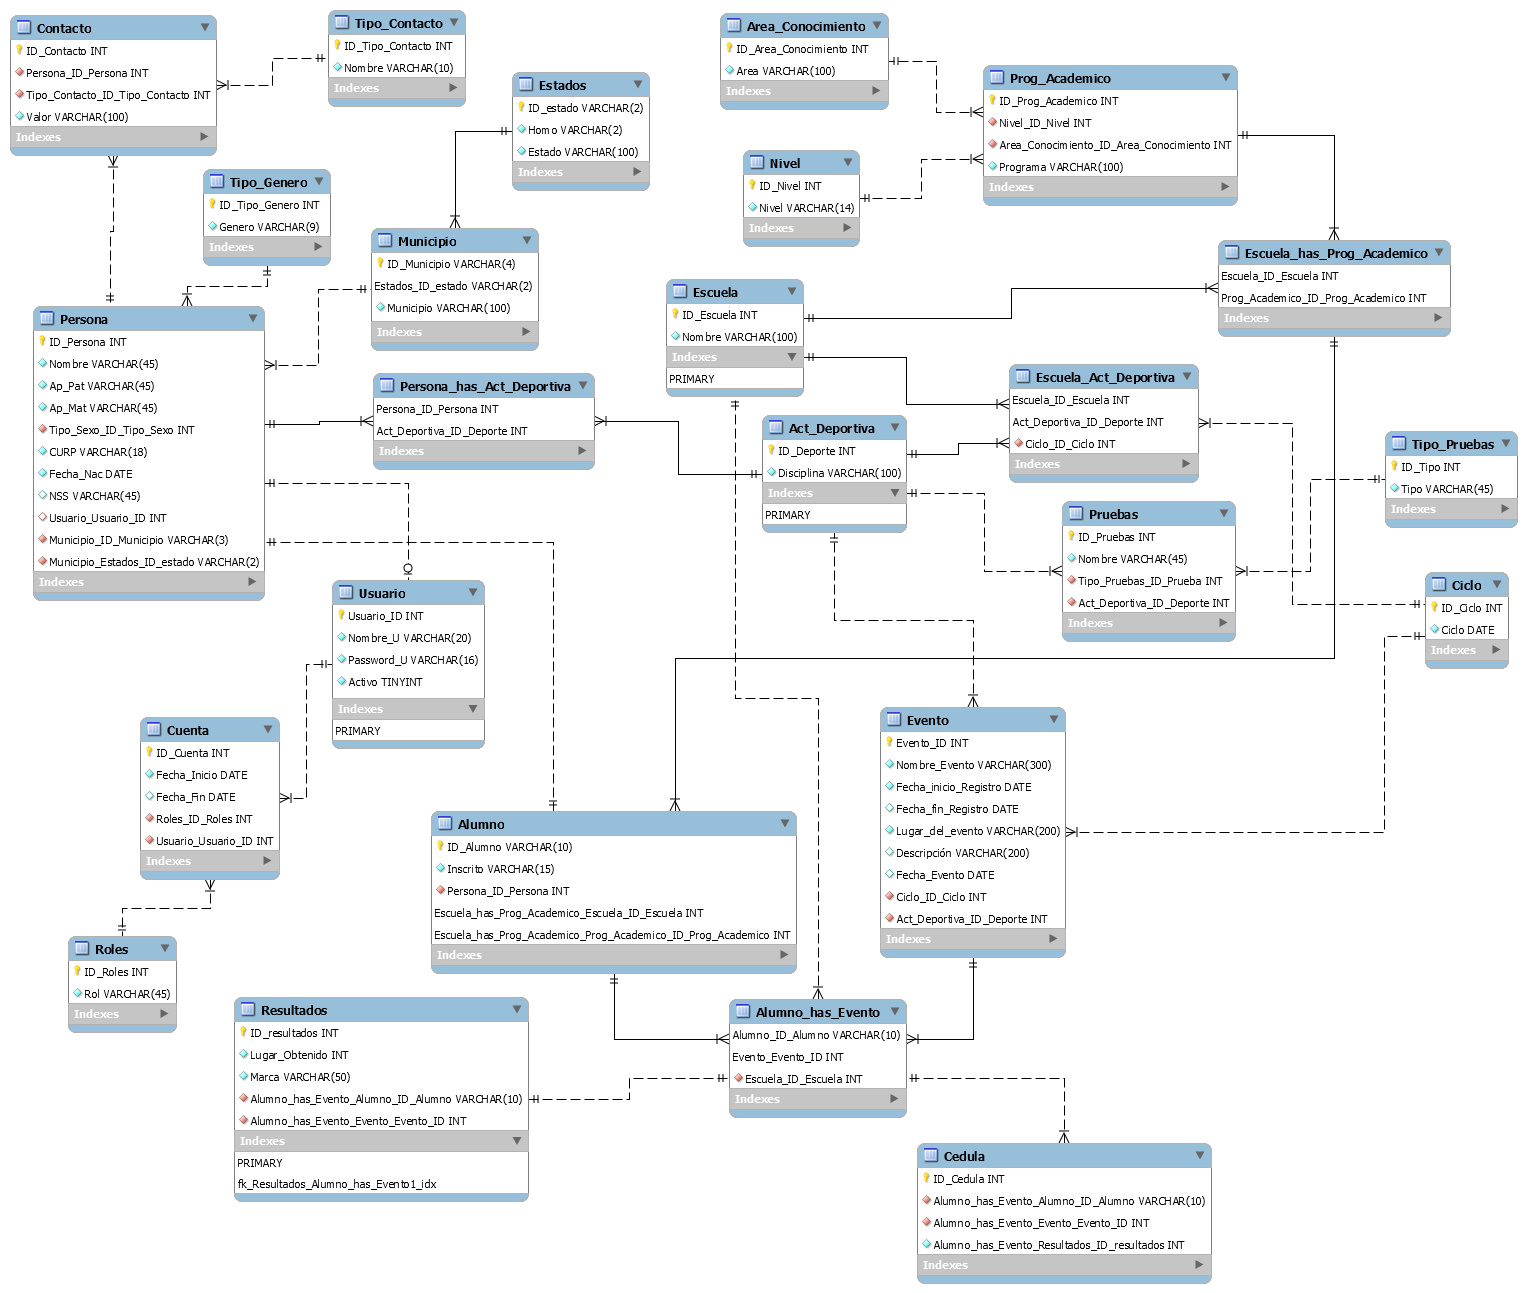
\includegraphics[width=22cm, height=15cm, angle=90]{Imagenes/BasedeDatos.png}
			\caption{Base de Datos}
		\end{figure}
	\end{enumerate}
	\pagebreak
	
	Como parte de la notación que se empleó 
	
	%=========================================================
	%                                                         Sprint 1
	%=========================================================
	\section{Sprint 1}
	El desarrollo de este SPRINT se consideró que la manera de validación del participante será que el alumno que desee participar en un evento interpolitécnico para ello deberá registrarse en la aplicación web posteriormente, deberá acudir con el coordinador de su Unidad Académica y que el corrobore sus datos solicitando alguna identificación, cabe destacar que este proceso de validación se hará solo una vez.
	Una vez que haya sido validado por el coordinador y este, activará su cuenta, el alumno interesado podrá ingresar en el sistema e inscribirse en una evento interpolitécnico dentro de las fechas establecidas.
	El objetivo de este mecanismo es comprobar la existencia de un alumno en la base de datos del plantel o en el IPN y aceptar únicamente a los que estén inscritos.
	
	
	%=========================================================
	%                                                         Sprint 2
	%=========================================================
	\section{Sprint 2}
	Para la desarrollo de este SPRINT se tomaron los debidos requerimientos para la realización del diseño de las interfaces y así hacer que la aplicación sea amigable con el usuario utilizando las siguientes plantillas para la visualización de las interfaces como una propuesta.
	
	Interfaz Inicio general: Esta interfaz es la principal donde los usuarios podrán visualizar datos de aspecto público. \newline
	Parte 1:
	Cualquier usuario que visite la URL de la aplicación podrá ver los elementos de navegación tales como: Inicio (Página principal), Registro, Calendario, Inicia Sesión, Contacto, los deportes que se imparten en la ESCOM, una introducción a los eventos interpolitécnicos deportivos próximos, como se muetra en la Figura 14. 
	\begin{figure}[hbt!]
		\centering
		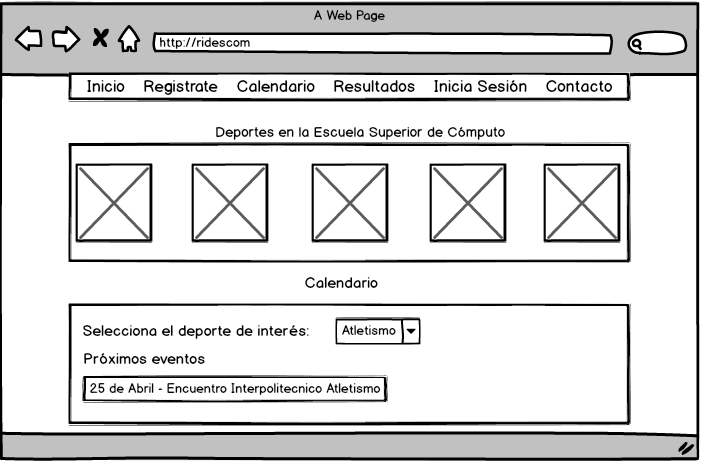
\includegraphics[width=10cm, height=6cm]{Imagenes/Disenos/Iniciogeneral.png}
		\caption{Página Inicio (comunidad en general)}
	\end{figure}
	Parte 2:
	Dentro de la misma habrá una sección de resultados generales de los últimos eventos realizados y finalmente una  sección donde se localiza el contacto del plantel para más información al respecto y un contacto de Facebook del área de actividades deportivas de la ESCOM, como se muetra en la Figura 15.
	\begin{figure}[hbt!]
		\centering
		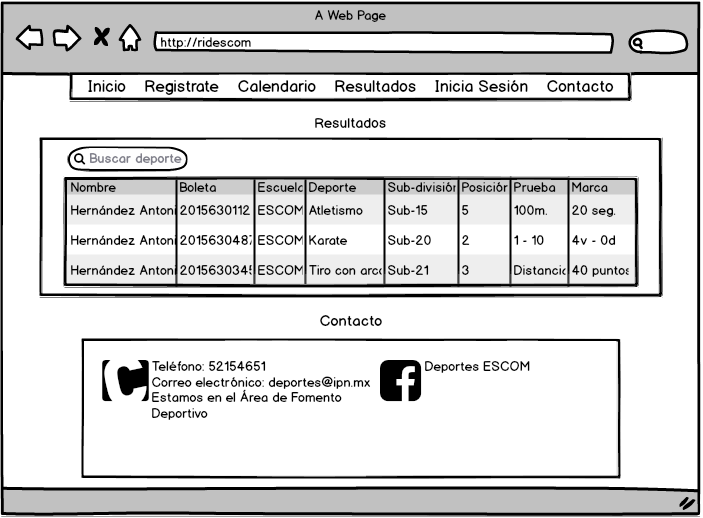
\includegraphics[width=10cm, height=6cm]{Imagenes/Disenos/Iniciogeneral1.png}
		\caption{Página Inicio 2 (comunidad en general)}
	\end{figure}
	\newline
	
	Interfaz Login: En esta interfaz ayuda al usuario indicando los elementos que se necesitan para iniciar sesión como usuario de la aplicación (Usuario/contraseña previamente registrado), si el usuario no existe el mecanismo realizado en el SPRINT1 se encargará de rechazarlo, podrá recuperar su contraseña en la sección de “¿Olvidaste tu contraseña?”, como se muestra en la Figura 16. \pagebreak
	\begin{figure}[hbt!]
		\centering
		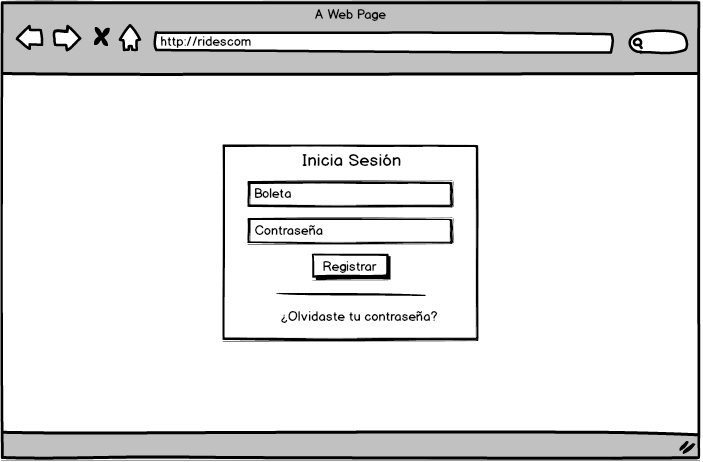
\includegraphics[width=10cm, height=6cm]{Imagenes/Disenos/Login.png}
		\caption{Login}
	\end{figure}
	
	Interfaz Registro: Para poder inscribirse en un interpolitécnico será necesario crear una cuenta en la aplicación, para esto se pedirán datos como la Boleta, un correo electrónico y una contraseña, como se muestra en la Figura 17.
	\begin{figure}[hbt!]
		\centering
		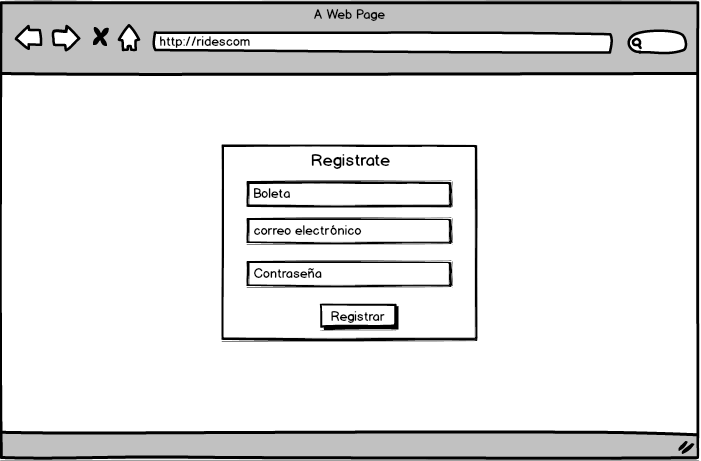
\includegraphics[width=10cm, height=6cm]{Imagenes/Disenos/Registro.png}
		\caption{Registro}
	\end{figure}
	\pagebreak
	
	Interfaz Recupera contraseña: En este módulo el participante (alumno) donde se le solicitará el correo electrónico para restablecer su contraseña, como se muestra en la Figura 18. 
	\begin{figure}[hbt!]
		\centering
		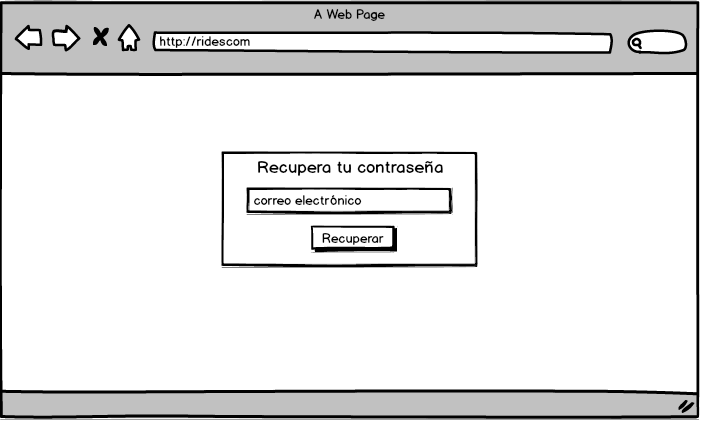
\includegraphics[width=10cm, height=6cm]{Imagenes/Disenos/Recuperacontrasena.png}
		\caption{Recupera contraseña}
	\end{figure}
	
	Interfaz Restablece contraseña: Una vez que se solicitará el recuperar la contraseña se enviará un link donde podrá ver una pantalla como se muestra en la Figura 18, solicitando ingresar una nueva contraseña y la confirmación de la misma, como se muestra en la Figura 19.
	\begin{figure}[hbt!]
		\centering
		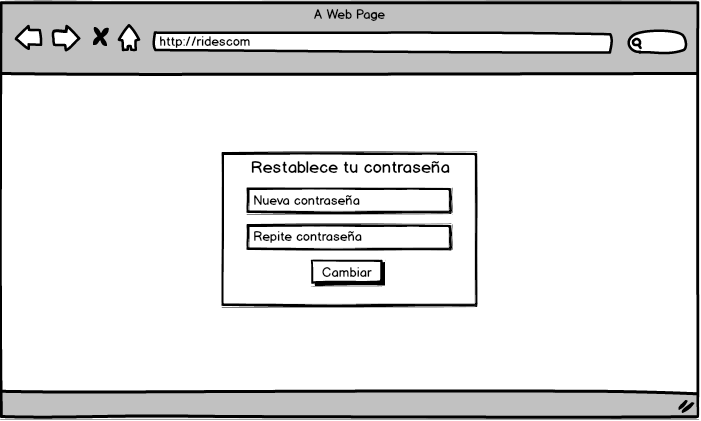
\includegraphics[width=10cm, height=6cm]{Imagenes/Disenos/Restablecercontra.png}
		\caption{Restablece contraseña}
	\end{figure}
	
	Interfaz Login del Jefe del Departamento de Fomento Deportivo: En esta interfaz ayuda al usuario indicando los elementos que se necesitan para iniciar sesión como usuario de la aplicación (Nombre-Usuario/contraseña previamente registrado), si el usuario no existe el mecanismo realizado en el SPRINT1 se encargará de rechazarlo, podrá recuperar su contraseña en la sección de “¿Olvidaste tu contraseña?”, como se muestra en la Figura 20.\pagebreak
	\begin{figure}[hbt!]
		\centering
		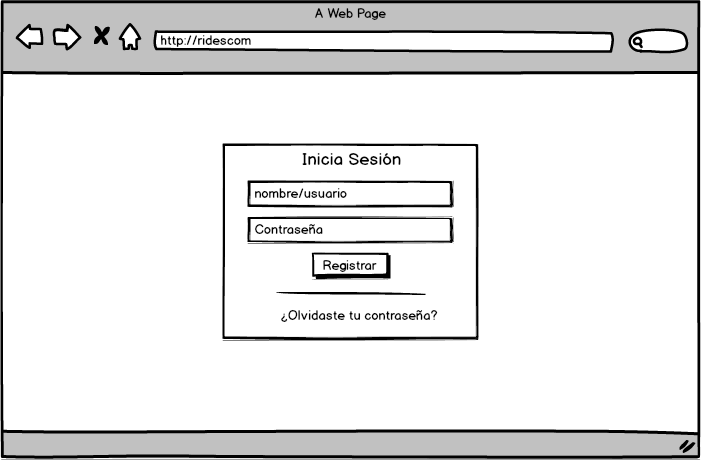
\includegraphics[width=10cm, height=6cm]{Imagenes/Disenos/LoginJFD.png}
		\caption{Login del Jefe del Departamento de Fomento Deportivo}
	\end{figure}
	
	Interfaz Inicio del Jefe del Departamento de Fomento Deportivo: El diseño de la página será muy similar con el resto de los usuarios, sin embargo, este contará con distintas opciones como son: Crear un evento deportivo, Resultados, Calendario y Control de cordinadores donde en este apartado tendrá la opción de Consultar coordinadores, Registrar usuario, Modificar contraseña de los coordinadores de las Unidades Académicas, como se muestra en la Figura 22. El diseño en general de la vista de este usuario se puede ver en  las Figuras 21 y 23.
	\begin{figure}[hbt!]
		\centering
		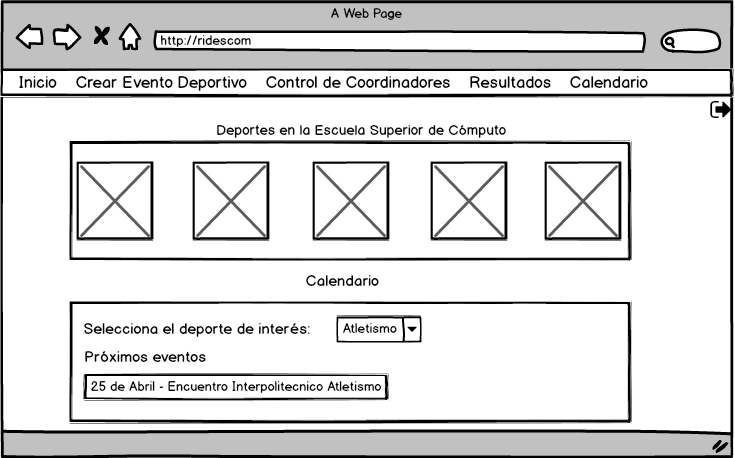
\includegraphics[width=10cm, height=6cm]{Imagenes/Disenos/InicioJFD.png}
		\caption{Página principal Jefe del Departamento de Fomento Deportivo}
	\end{figure}
	
	\pagebreak
	
	\begin{figure}[hbt!]
		\centering
		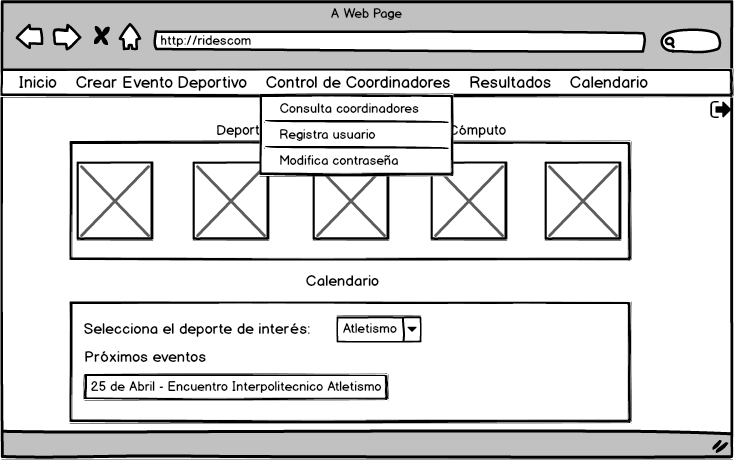
\includegraphics[width=10cm, height=6cm]{Imagenes/Disenos/InicioJFDopciones.png}
		\caption{Página principal Jefe del Departamento de Fomento Deportivo}
	\end{figure}
	\begin{figure}[hbt!]
		\centering
		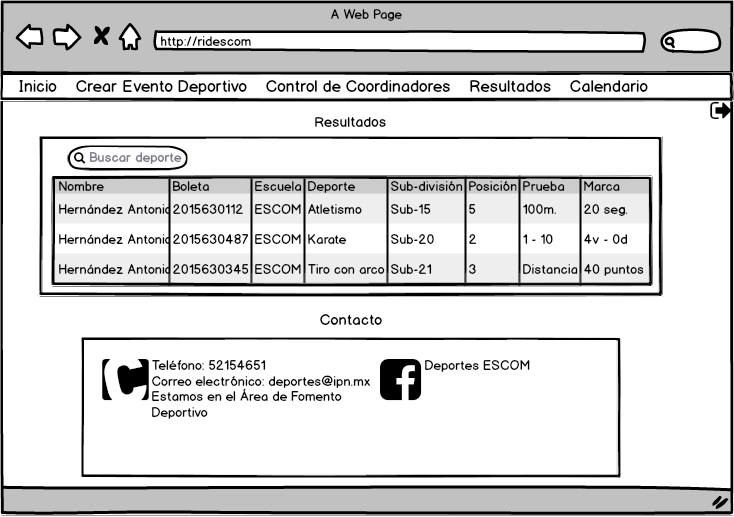
\includegraphics[width=10cm, height=6cm]{Imagenes/Disenos/Inicio1JFD.png}
		\caption{Página principal del Jefe del Departamento de Fomento Deportivo 1}
	\end{figure}
	
	Interfaz Crear un evento interpolitécnico: Dentro de esta vista el Jefe del Departamento de Fomento Deportivo llenaráa los campos para poder dar de alta algún evento, se pedirá el Nombre del evento, Fecha en la que se llevará acabo, Fecha inicio de inscripción y Fecha fin de inscripción, un campo de Descripción donde podrá agregar la dirección del lugar entre otros datos. Se seleccionará el deporte al que corresponde dicho evento, así como la Sub-división y Prueba, como se muestra en la Figura 24.
	\pagebreak
	\begin{figure}[hbt!]
		\centering
		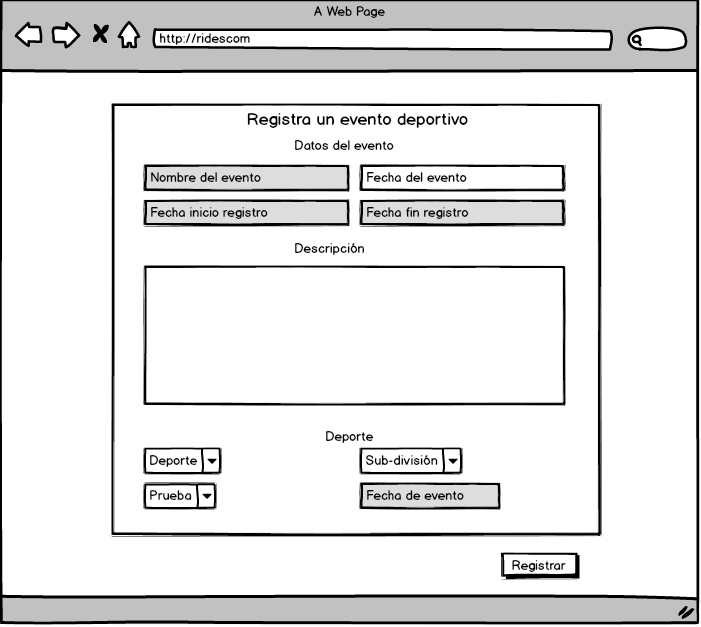
\includegraphics[width=10cm, height=6cm]{Imagenes/Disenos/Registrauneventodeportivo.png}
		\caption{Crear un evento deportivo}
	\end{figure}
	
	Interfaz Registra un coordinador: Se solicitarán datos como Nombre, Apellido Paterno, Apellido Materno,correo electrónico, teleéfonos de contacto y Escuela a la que pertenece, como se muestra en la Figura 25.
	\begin{figure}[hbt!]
		\centering
		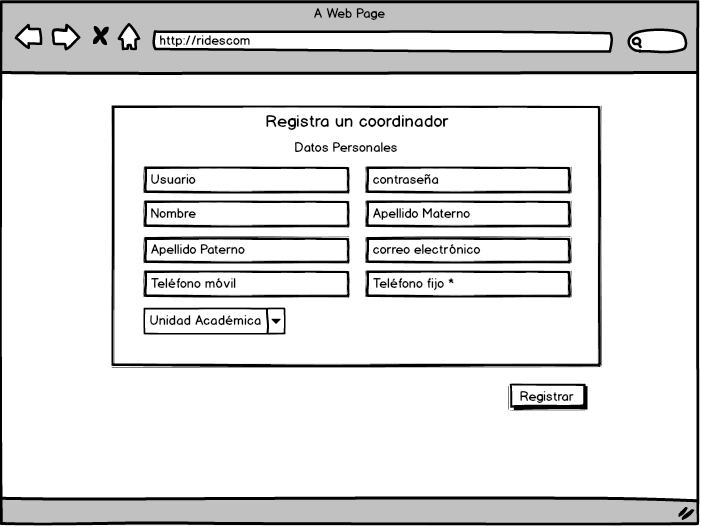
\includegraphics[width=10cm, height=6cm]{Imagenes/Disenos/Registrocoordinador.png}
		\caption{Registra un coordinador}
	\end{figure}
	
	Interfaz login coordinador: En esta interfaz ayuda al usuario indicando los elementos que se necesitan para iniciar sesión como usuario de la aplicación (Nombre-Usuario/contraseña previamente registrado), si el usuario no existe el mecanismo realizado en el SPRINT1 se encargará de rechazarlo, como se muestra en la Figura 26. En caso de que el coordinador olvide su contraseña deberá ponerse en contacto con el Jefe del Departamento de Fomento Deportivo para solicitar el cambio de contraseña \pagebreak
	\begin{figure}[hbt!]
		\centering
		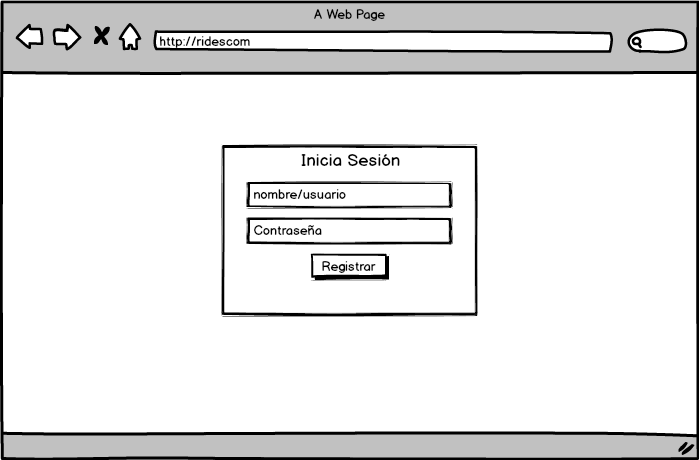
\includegraphics[width=10cm, height=6cm]{Imagenes/Disenos/LogincoordinadorUA.png}
		\caption{Login para el coordinador de la Unidad Académica}
	\end{figure}
	
	Interfaz  Inicio del coordinador de una Unidad Académica: Al igual que el resto de los usuarios en general tiene un diseño muy similar, la diferencia recae en las opciones que puede realizar, en este caso son: Registrar entrenador, Calendario, Resultados, Consulta de inscripciones y Válidar perfil, como se muestra en las Figura 27 y en la Figura 28 se puede observar que estará disponible un apartado para publicar algun evento previamente dado de alta en la red social de Facebook.
	
	\begin{figure}[hbt!]
		\centering
		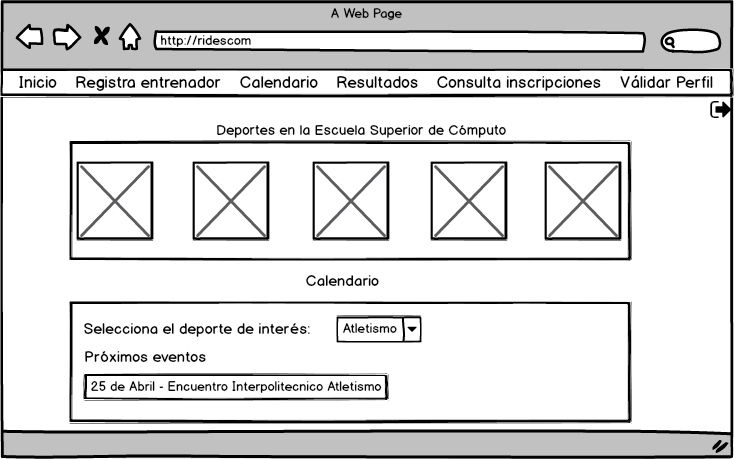
\includegraphics[width=10cm, height=6cm]{Imagenes/Disenos/IniciocoordinadorUA.png}
		\caption{Página principal del coordinador de la Unidad Académica}
	\end{figure}
	
	\pagebreak
	
	\begin{figure}[hbt!]
		\centering
		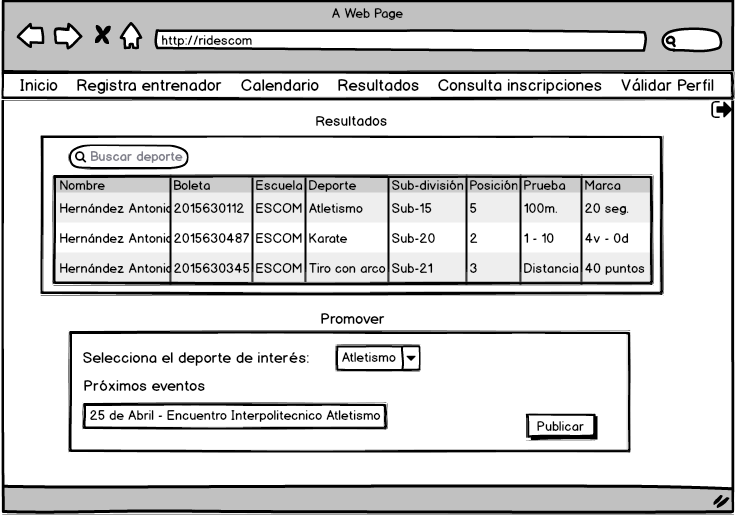
\includegraphics[width=10cm, height=6cm]{Imagenes/Disenos/IniciocoordinadorUA1.png}
		\caption{Página principal del coordinador de la Unidad Académica 1}
	\end{figure}
	
	Interfaz Registro entrenador: En este  módulo el coordinador deberá los campos solicitados tales como: No. Empleado, Nombre, Apellidos, Correo electrónico, Teléfono fijo, Teléfono móvil, asi como definir a que deporte pertenece y por ultimo, especificar si cuenta con un asistente, como se muestra en la Figura 29.
	\begin{figure}[hbt!]
		\centering
		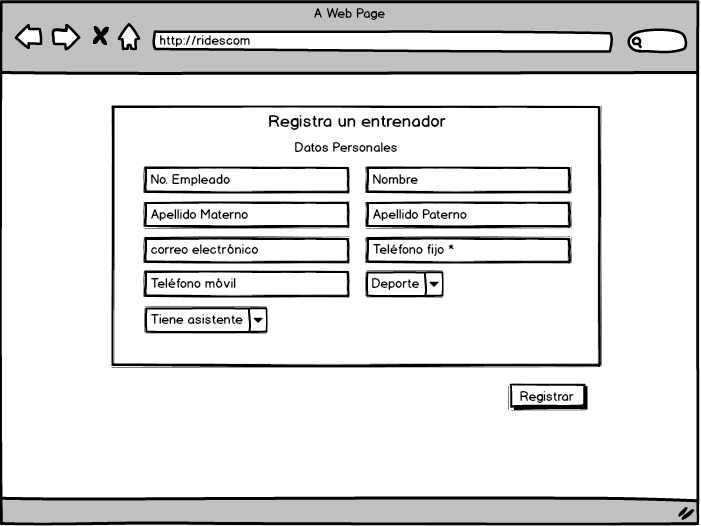
\includegraphics[width=10cm, height=6cm]{Imagenes/Disenos/Registraunentrenador.png}
		\caption{Registra un entrenador}
	\end{figure}
	
	Interfaz Válidar un perfil: Este módulo servirá como un filtro para verificar que la persona que esta solicitando crear su perfil en la aplicación, sea quién dice ser. Cabe destacar que dicha validación se realizará una sola vez. Una vez que el alumno se presente con el coordinador, este solicitará una identificación para válidar los datos, si cumple podrá activar el perfil del usuario, como se muestra en la Figura 30.
	\begin{figure}[hbt!]
		\centering
		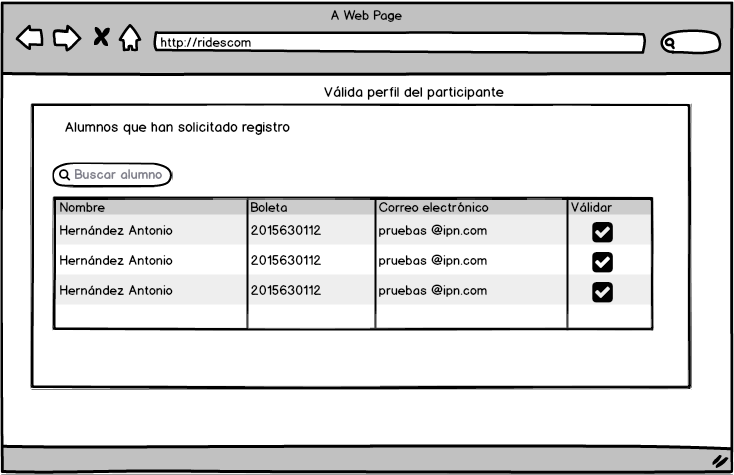
\includegraphics[width=10cm, height=6cm]{Imagenes/Disenos/Validaperfil.png}
		\caption{Válidar un perfil}
	\end{figure}
	\pagebreak
	
	Interfaz Resultados: Este módulo esta designado para que se ingresen los resultados de los participantes y sean vistos en la página principal. Podrá ingresar hasta 20 datos por vez, como se muestra en la Figura 31.
	\begin{figure}[hbt!]
		\centering
		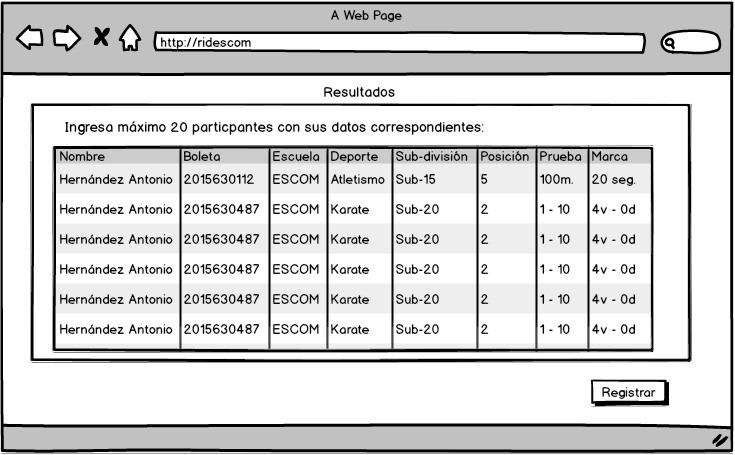
\includegraphics[width=10cm, height=6cm]{Imagenes/Disenos/Ingresaresultados.png}
		\caption{Ingresa resultados de los eventos}
	\end{figure}
	\pagebreak
	
	Interfaz Inicio del participante: El diseño de la página será muy similar con el resto de los usuarios, sin embargo, este contará con distintas opciones como son: Inscribir un Interpolitécnico, Calendario, Consulta tus registros y Contacto, como se muestra en la Figura 21. El diseño en general de la vista de este usuario se puede ver en  las Figuras 32 y 33.
	\begin{figure}[hbt!]
		\centering
		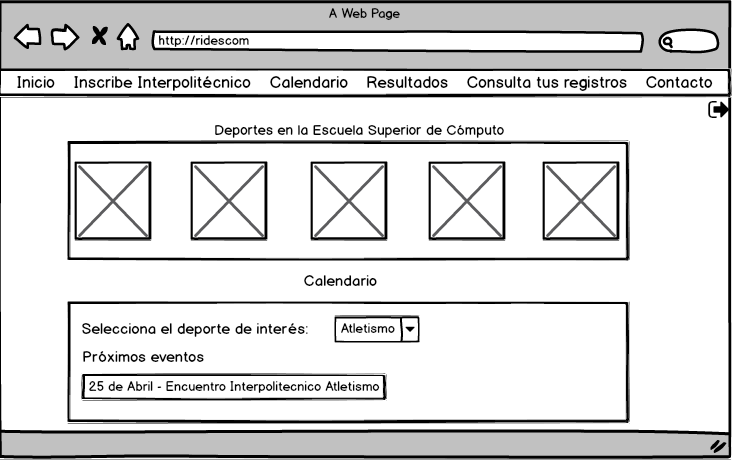
\includegraphics[width=10cm, height=6cm]{Imagenes/Disenos/Inicioparticipante.png}
		\caption{Página principal del participante}
	\end{figure}
	\begin{figure}[hbt!]
		\centering
		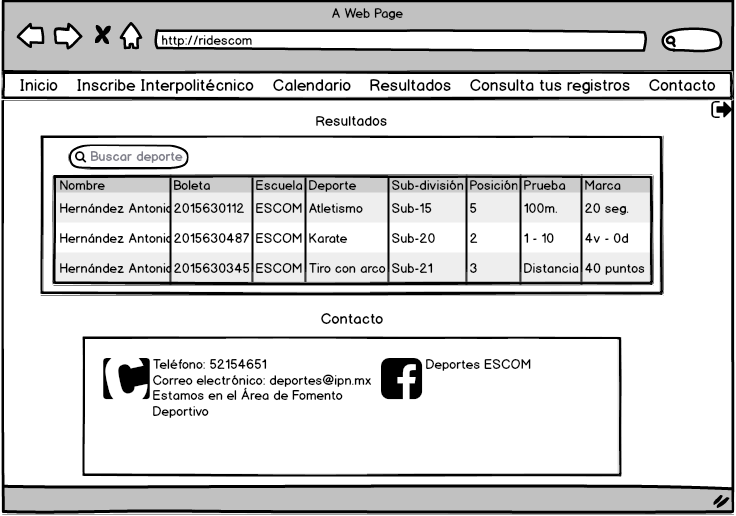
\includegraphics[width=10cm, height=6cm]{Imagenes/Disenos/Inicioparticipante1.png}
		\caption{Página principal del participante 1}
	\end{figure}
	
	Interfaz Inscribir interpolitécnico: En este módulo el alumno primero deberá válidar el estatus de su inscripción, si esta inscrito en el periodo actual, se habilitará el botón para registrar la cédula. En caso contrario el botón no estará habilitado y por tanto, no podrá inscribirse. Los campos que debera llenar el alumno serán: Grupo, NSS (Número de Seguro Social), Lugar de Nacimiento, correo electrónico, Delegación/Municipio, asi como seleccionar el deporte, sub-division y prueba en la que quiere participar, como se muestra en la Figura 34.
	\begin{figure}[hbt!]
		\centering
		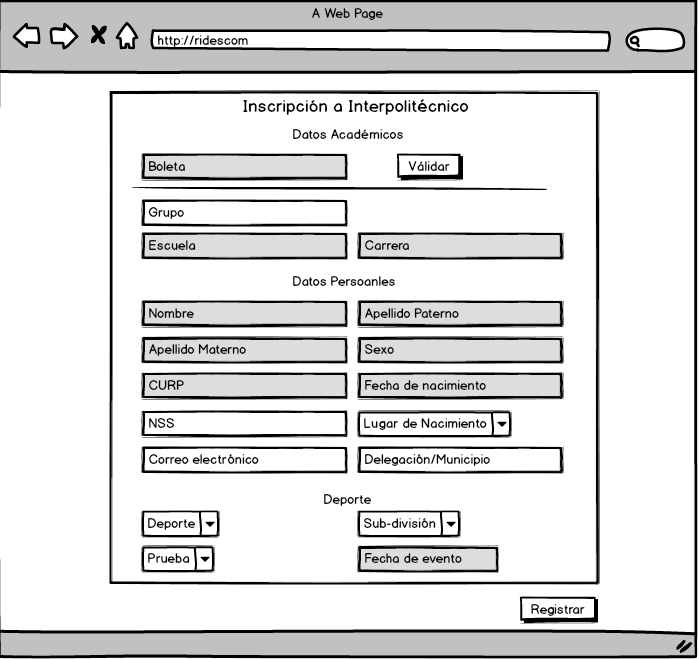
\includegraphics[width=10cm, height=6cm]{Imagenes/Disenos/Inscripcioninter.png}
		\caption{Inscribir un interpolitécnico}
	\end{figure}
	\pagebreak
	
	Interfaz Consulta tus registros: En este módulo, el participante podrá visualizar en una tabla los eventos a los cuales se a registrado, a su vez le mostrará información como: el deporte, prueba Fecha del Evento y la direccion del mismo, como se muestra en la Figura 35.
	\begin{figure}[hbt!]
		\centering
		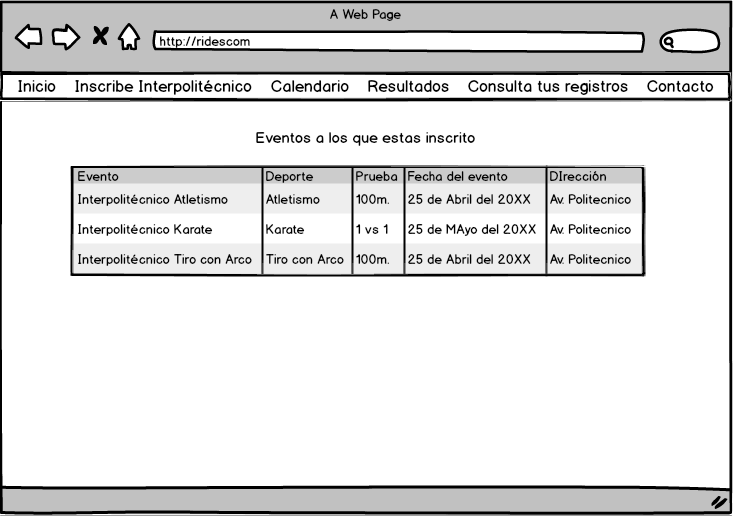
\includegraphics[width=10cm, height=6cm]{Imagenes/Disenos/Consultainscripciones.png}
		\caption{Consulta eventos a los que se ha registrado}
	\end{figure}
	
	
	%=========================================================
	%                                                         Sprint 3
	%=========================================================
	\section{Sprint 3}
	
	%=========================================================
	%                                                         Sprint 4
	%=========================================================
	\section{Sprint 4}
	
	%=========================================================
	%                                                         Sprint 5
	%=========================================================
	\section{Sprint 5}
	
	%=========================================================
	%                                                         Sprint 6
	%=========================================================
	\section{Sprint 6}
	
	%=========================================================
	%                                                         Sprint 7
	%=========================================================
	\section{Sprint 7}
	